\section{OWL Verbalizer}
OWL~Verbalizer~\cite{stevens2011}, an open source tool aimed at producing texts from generic OWL ontologies, is a good example of a successful integration of ACE. A description of the basic concepts of OWL Verbaliser is given below:

This tool, being now part of the \textbf{SWAT Tool Suite}\footnote{\url{http://mcs.open.ac.uk/nlg/SWAT/} accessed 2018/05/06}, was created to overcome the burden of maintaining ontology definitions by hand. Whereas producing high quality texts in restricted application domains is under active research, this tool produces understandable descriptions using general-purpose methods that are of moderate quality.

The high-level process of ontology verbalisation shown in \hyperref[fig:verbaliser_architecture]{Figure~\ref*{fig:verbaliser_architecture}} consists of the following stages:

\paragraph{Transcoding from OWL to Prolog} The output of this stage is a file in a convenient Prolog format which was generated from an ontology in RDF/XML format. The conversation process covered by the \textit{Transcoder}, \textit{Identifier~Selector} and \textit{Label~Selector} combines identifiers~(concepts, individuals, object~properties) and labels. In addition, ambiguous terms in identifiers are normalised. 

\paragraph{Constructing a lexicon for atomic entities} The output of this stage, covered by the component \textit{Lexicon Generator}, is a collection of lexicons, computed from the normalised Prolog terms in the previous stage. A lexical entry~(lexicon) is defined as a quadruple having the following form: \texttt{<identifier, part-of-speech, singular-form, plural-form>} To facilitate processing in later stages, normalised identifiers for concepts, individuals and object~properties are stored together with word category, singular form and plural form. The word~category, also known as part-of-speech, groups words based on similar properties in terms of syntax and grammar. Common categories are nouns, verbs and adjectives. Last, to differentiate the quantity of a phrase or word, singular and plural form of a noun are associated with each lexical entry. 
Among the storage of lexicons, the algorithm also implements other rules regarding text processing. Some simple heuristics are used for pre-processing to transform the resulting word string into better readable English sentences. 

\paragraph{Selecting the axioms relevant for describing each class} This stage and the next stage are covered by the \textit{Planner}.
This component has as input all axioms from the source ontology as well as the lexicons from the previous stage. In this stage, axioms are mapped to matching lexical entries. As matching criteria the algorithm uses the lexicon identifier and the IRI~\cite{rfc3987}. 

\paragraph{Aggregating axioms with a similar structure} This stage is optional, as it is not strictly required for text generation which is described in the next stage. However, some improvements are achieved if similar axioms are aligned. 

\paragraph{Generating sentences from axioms} The final stage is covered by the component named \textit{Realiser} which forms the central part of the
verbalisation process. English sentences are generated for each axiom using logical rules for almost every logical pattern in OWL-DL. These rules are expressed in Prolog clauses, taking the axiom and optionally the lexicon as input.

\begin{figure}
	 \centering
	 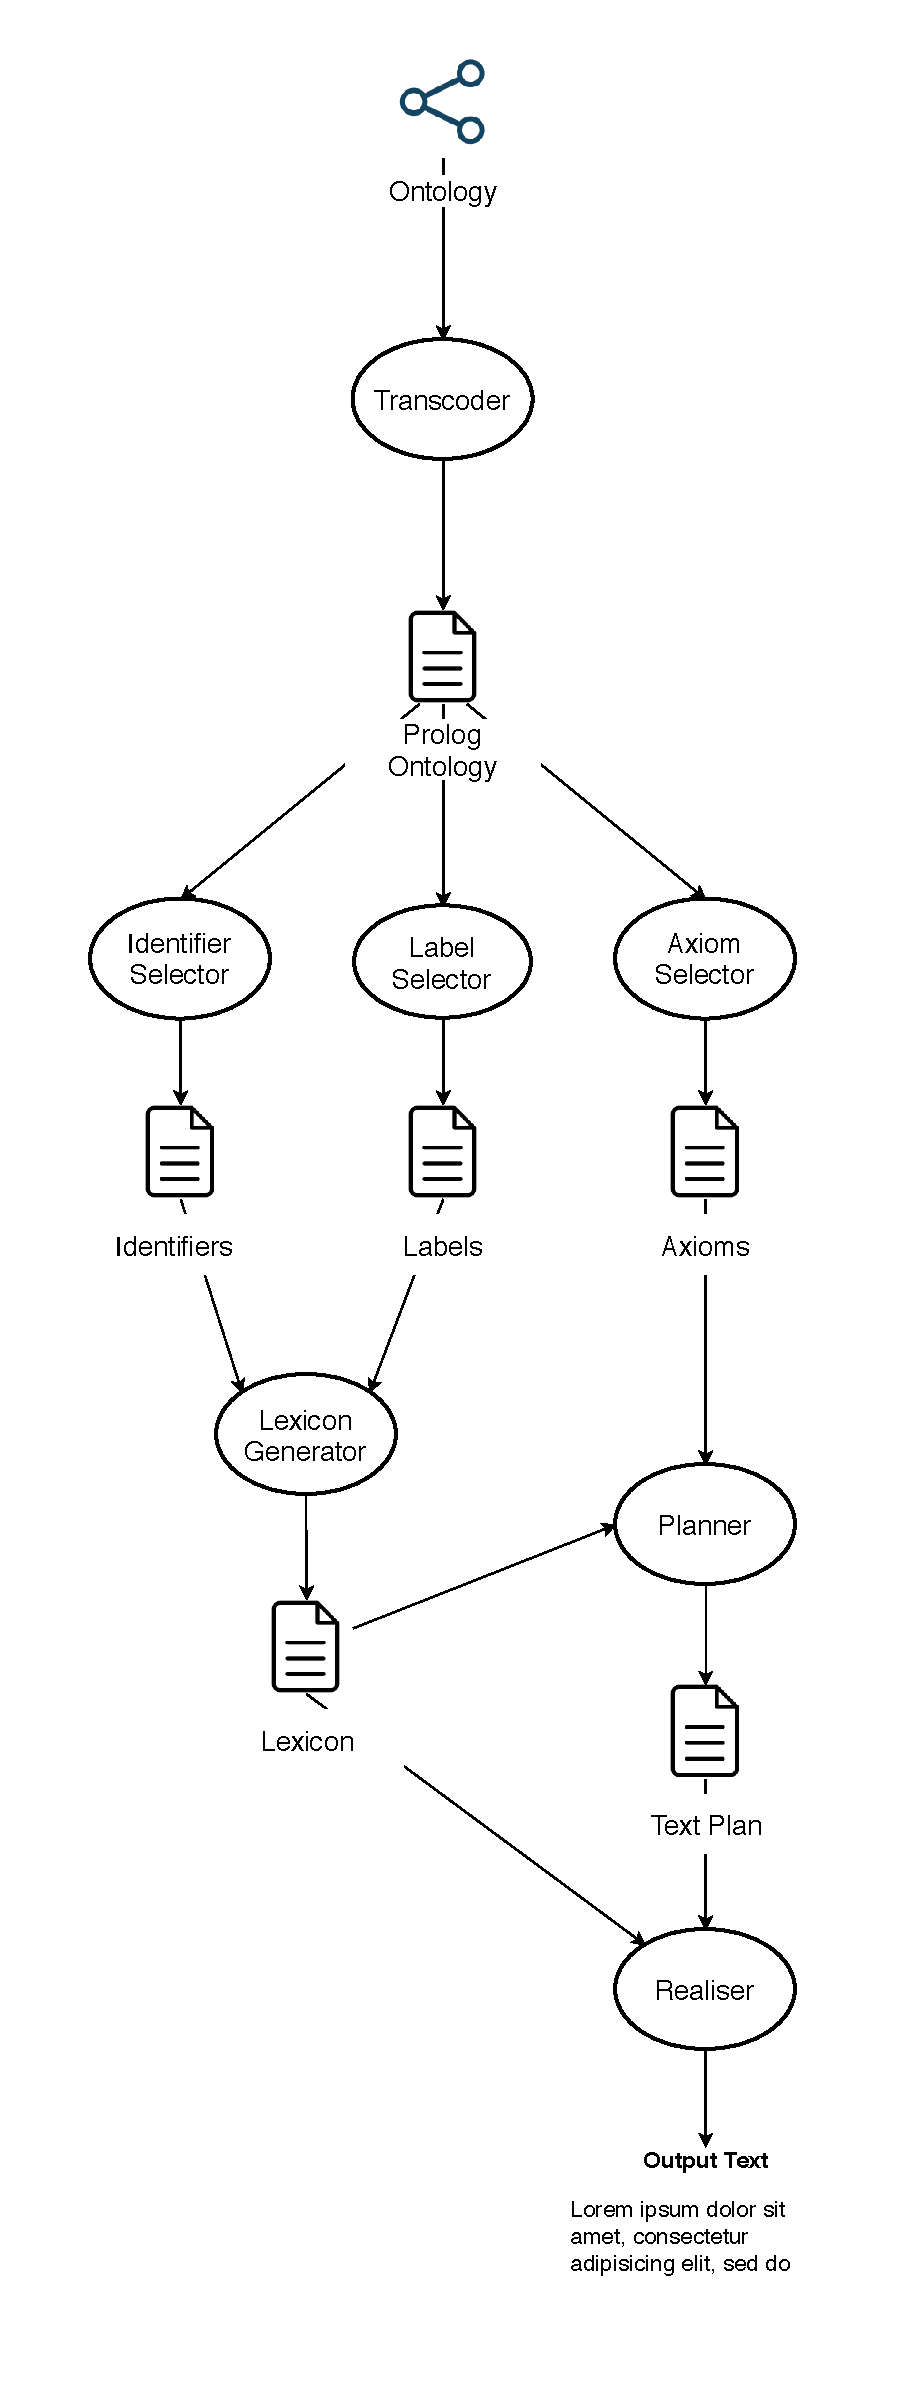
\includegraphics[width=0.5\textwidth]{drawio/Ontology_Verbaliser_Architecture}
	 \caption{Conceptual architecture of the OWL ontology verbaliser~\cite{stevens2011}}\label{fig:verbaliser_architecture}
\end{figure}

Although OWL~Verbaliser would be useful to integrate in the enrichment process, there are some major obstacles:

The first is \textbf{incompatibility on a language level}. Traditionally, software systems are written in many different programming languages, leading to the challenge of dealing with interoperability~\cite{malone2014}. While OWL~Verbaliser was written in SWI-Prolog, Protege runs on the Java Virtual Machine~(JVM), causing a conceptual mismatch in programming languages and paradigms. Moreover, interoperability between conceptually different programming languages is challenging in its own\footnote{\url{http://www.swi-prolog.org/packages/jpl/} accessed 2018/05/11} and would conflict with the goal of an easy-to-integrate solution.

Another obstacle is a \textbf{mismatch on the scope of operation}. OWL~Verbaliser was implemented as a tool assisting engineers in ontology creation, a very time consuming task. It was designed as a standalone tool, launched from the command line or deployed as a web service. On the other hand, ontology enrichment is embedded in Protege and part of the ontology validation process, operating only on small parts of the ontology. In contrast, OWL~Verbaliser takes the whole ontology as input. 
